\documentclass{article}
\usepackage{amsmath,amsfonts,amsthm,amssymb}
\usepackage{setspace}
\usepackage{fancyhdr}
\usepackage{mathrsfs}
\usepackage{lastpage}
\usepackage{extramarks}
\usepackage{chngpage}
\usepackage{soul,color}
\usepackage{graphicx,float,wrapfig}
\usepackage{CJK}
\usepackage{algorithm}
\usepackage{algorithmic}
\usepackage{graphicx}
\newcommand{\Class}{Distributed System}

% Homework Specific Information. Change it to your own
\newcommand{\Title}{Project 2 Report}

% In case you need to adjust margins:
\topmargin=-0.45in      %
\evensidemargin=0in     %
\oddsidemargin=0in      %
\textwidth=6.5in        %
\textheight=9.0in       %
\headsep=0.25in         %

% Setup the header and footer
\pagestyle{fancy}                                               %
\chead{\Title}  %
\rhead{\firstxmark}                                                     %
\lfoot{\lastxmark}                                                      %
\cfoot{}                                                                %
\rfoot{Page\ \thepage\ of\ \protect\pageref{LastPage}}                          %
\renewcommand\headrulewidth{0.4pt}                                      %
\renewcommand\footrulewidth{0.4pt}                                      %

%%%%%%%%%%%%%%%%%%%%%%%%%%%%%%%%%%%%%%%%%%%%%%%%%%%%%%%%%%%%%
% Some tools
\newcommand{\enterProblemHeader}[1]{\nobreak\extramarks{#1}{#1 continued on next page\ldots}\nobreak%
	\nobreak\extramarks{#1 (continued)}{#1 continued on next page\ldots}\nobreak}%
\newcommand{\exitProblemHeader}[1]{\nobreak\extramarks{#1 (continued)}{#1 continued on next page\ldots}\nobreak%
	\nobreak\extramarks{#1}{}\nobreak}%

\newcommand{\homeworkProblemName}{}%
\newcounter{homeworkProblemCounter}%
\newenvironment{homeworkProblem}[1][Problem \arabic{homeworkProblemCounter}]%
{\stepcounter{homeworkProblemCounter}%
	\renewcommand{\homeworkProblemName}{#1}%
	\section*{\homeworkProblemName}%
	\enterProblemHeader{\homeworkProblemName}}%
{\exitProblemHeader{\homeworkProblemName}}%

\newcommand{\homeworkSectionName}{}%
\newlength{\homeworkSectionLabelLength}{}%
\newenvironment{homeworkSection}[1]%
{% We put this space here to make sure we're not connected to the above.
	
	\renewcommand{\homeworkSectionName}{#1}%
	\settowidth{\homeworkSectionLabelLength}{\homeworkSectionName}%
	\addtolength{\homeworkSectionLabelLength}{0.25in}%
	\changetext{}{-\homeworkSectionLabelLength}{}{}{}%
	\subsection*{\homeworkSectionName}%
	\enterProblemHeader{\homeworkProblemName\ [\homeworkSectionName]}}%
{\enterProblemHeader{\homeworkProblemName}%
	
	% We put the blank space above in order to make sure this margin
	% change doesn't happen too soon.
	\changetext{}{+\homeworkSectionLabelLength}{}{}{}}%

\newcommand{\Answer}{\ \\\textbf{Answer:} }
\newcommand{\Acknowledgement}[1]{\ \\{\bf Acknowledgement:} #1}

%%%%%%%%%%%%%%%%%%%%%%%%%%%%%%%%%%%%%%%%%%%%%%%%%%%%%%%%%%%%%


%%%%%%%%%%%%%%%%%%%%%%%%%%%%%%%%%%%%%%%%%%%%%%%%%%%%%%%%%%%%%
% Make title
\title{\textmd{\bf \Class: \Title}\\ \normalsize\vspace{0.1in}}
\date{}
%%%%%%%%%%%%%%%%%%%%%%%%%%%%%%%%%%%%%%%%%%%%%%%%%%%%%%%%%%%%%

\begin{document}
	\begin{spacing}{1.0}
		\maketitle \thispagestyle{empty}

		\section{Part1: Implementation Details}
		\subsection{Client}
		The code for \texttt{Client} is mainly in \textit{client.go}, which is acting like an test file. In that file, you will create some \texttt{wallet} and define their actions like ``A transfer AMOUNT to B''.
		Since our implementation is based on UTXOSet, the transaction should includes multiple \texttt{TxIn} and multiple \texttt{TxOut} (explained later). In our implementation, a wallet will not maintain a 
		\texttt{UTXOSet} it self, he needs to get one from one \texttt{Miner} and then create corresponding \texttt{Transaction}s (find enough his spendable \texttt{TxOut} in the UTXOSet for the AMOUNT it needs). Also, 
		he need to sign the inputs of the transaction. After that, he needs to broadcast all the transactions to all the miners.

		\subsection{Wallet}
		The code for \texttt{Wallet} is mainly in \textit{wallet.go}. A wallet consists of a pair of (PublicKey, PrivateKey). And we identify each wallet by the hash of its PublicKey.

		\subsection{TxIn}
		The code for \texttt{TxIn} is mainly in \textit{TxIn.go}. It is just a struct containing the signature and PublicKey (used to verify the legal wallet), the \texttt{TxOut} it is using.

		\subsection{TxOut}
		The code for \texttt{TxOut} is mainly in \textit{TxOut.go}. It contains the value of this output and the target wallet's PublicKeyHash (used to specify to whom).

		\subsection{Transaction}
		The code for \texttt{Transaction} is mainly in \textit{Transaction.go}. There are basicly two types of transactions. One is called ``CoinBaseTransaction'', which has no input and is used to generate some initial \texttt{TxOut}. Another is 
		the normal transactions that are raised by wallets to spend their spendable outputs.
		When creating a normal transaction, a wallet need to sign on every input of the transaction using its PublicKey and specify the receiver by putting the receiver's PublicKeyHash in the output.
		
		\subsection{Block}
		The code for \texttt{Block} is mainly in \textit{block.go}. For each block, it contains ``Header'': the hash value of the transactions, ``PrevHash'': the hash value of the previous block, ``ID'': the height of this block, 
		``TimeStamp'': the time when this block is created, ``Nonce'': the result of ProofOfWork, ``Transactions'': the list of all the transactions kept in this block. The block need to make sure that the hash of the contatenate of the hash of this block (all the stuff, including the nounce) and the nounce should have enough number of leading zeros.


		\subsection{BlockChain}
		The code for \texttt{BlockChain} is mainly in \textit{blockchain.go}. It contains an array of blocks, making sure that they are linked by PrevHash.

		\subsection{UTXOSet}
		The code for \texttt{UTXOSet} is mainly in \textit{UTXOset.go}. It contains a map with key being the PublicKeyHash, representing each wallet and value being a list of his spendable \texttt{TxOut}.

		\subsection{Miner}
		The code for \texttt{Miner} is mainly in \textit{miner.go}. It contains one \texttt{UTXOSet}, one \texttt{Blockchain} and several channels used to transmit information. We are making sure that the Blockchain and the UTXOSet it contains are consistent, i.e. all the spendable TxOut in the 
		UTXOSet have not been used in the Blockchain or the set of transactions it is working on, and you can find those TxOut in the Blockchain or the set of transactions it is working on. Below shows our method.
		\subsubsection{Receive a transaction from the client:} When receiving a transaction from the client, the miner first check that the validation of the transaction (signature, amount ...) and all the inputs are in UTXOSet. Then he interrupt the mining process, update the UTXOSet by the content of this transaction, put this transaction into the block he's mining and restart the mining process.
		After mined out one block, it will broadcast the block to all miners.
		\subsubsection{Receive a block from another miner:} When a miner gets a new block and send it to me, I will first check the validation of this block (if invalid, just ignore it) and then check whether the PrevHash of the block is the hash of the tailblock of my blockchain. 
		
		If yes, it means that 
		our blockchains are the same (except for the sent block), hence this block is also legal in my blockchain. Then I will undo the update of UTXOSet of the current transactions I am working on, update all the transactions in this block and then reverify the transactions I was working on and update the UTXOSet by the content of those legal transactions (ignore the illegal transactions).
		
		If not, it means that our blockchains differ. We should adopt ``Longest Chain Rule''. If your block's ID is smaller than or equal to mine, I will just ignore this block. If your ID is greater (your chain is longer), I will send a request for your whole chain. By scaning over the PrevHash in chain, we can find the first different block and then check whether your blocks are valid (PrevHash correct, PoW correst). If your chain is 
		indeed valid, I will undo the update of UTXOSet of my blocks and the transactions I am current working on. Append your blocks to my chain and update the UTXOSet by the contents. Then we will redo all the transactions undone just now (verify whether they are legal according to current UTXOSet and decide whether to work on it) and further keep on mining.


		\section{Part1: Attack and Defense}
		There are several kinds of attack we can defend:
		\begin{itemize}
			\item Wallet fake on the amount of Transactions. We will verify the amount of the transaction when the miner get the transaction from the client. If sum(input) $<$ sum(output), it will output ``Not Enough Inputs! Fake Client !!!'' and ignore the transaction.
			\item Wallet fake on the signature. Verified when the miner get the transaction from the client, output `` Wrong Signature! Fake Client !!!'' and ignore the transaction
			\item Miner fake on ProofOfWork. When a miner get a block from another miner, it will verify its PoW, if fake, raise ``Invalid Block'' and ignore this block.
			\item Miner fake on PrevHash. When a miner get the blockchain from another miner (want to adopt ``longest chain rule''), it needs to verify that the chain is valid 
			on the PrevHash pointers. If we find that the blockchain is invalid, we will just take the miner as a lyer and ignore his blockchain and keep working on our own work.
		\end{itemize}
		Notice that there is another kind of attack: a miner fake on transactions it have mined out (only change the content of the transaction but the PrevHash, PoW are correct). Up to now, we assume that 
		our miner will only put the transactions permitted by his own UTXOSet onto his blockchain. In this setting, this attack will not be raised so we cannot handle this so far. We may fix this problem in Part2. 

		\section{Part2: Improvements}
		\subsection{Merkel Tree}
		We change the structure of a block, and set the header of block to be the root of merkel tree built from transactions in it.
		When the block is printed out in terminal, the tree will also be printed out like below:
		\begin{figure}[htbp]
			\centering
			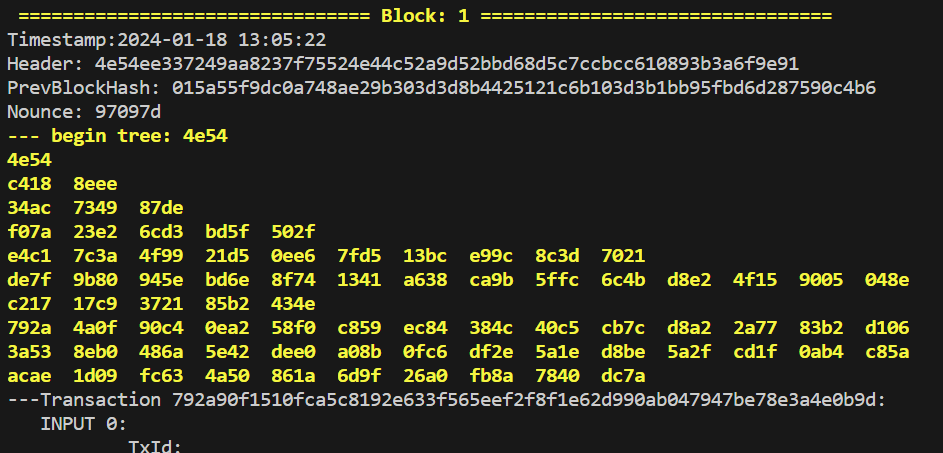
\includegraphics[width=0.9\textwidth]{./Merkel-Tree.png}
			\caption{figure for section 2}
		\end{figure}
		\subsection{Dynamic List of Miner}
		We add two grpc protocols to achieve this. First each miner maintains a list of address which it can communicate with.
		When a miner is added, it needs to know the address of at least one miner. This is achieved in function `GetAddrList'. Then it will call these existing miners to 
		get their address list and set its own list to be the union of these lists. After this, it will send its own address to the address in its own list
		to let these miners add its address to their list. This is achieved in function `UpdateAddrList'.
		\subsection{Disable the attack of fake transactions}
		In the Attack and Defense part we mentioned that we assume the miner will not include transactions that can not be done in its own UTXO set.\\
		Now we remove the assumption. \\
		When a miner receives a block, we need to simulate the transactions of incoming block in its own UTXO set. If one of the transaction cannot be done, then 
		we will undo the previous simulated transactions and reject the block. So is for the case when miner gets a chain from other miners, but in this case we will first 
		undo the blocks different from the incoming blockchain, then simulate the different part of incoming chain, if simulation fails (one transaction cannot be done), then we
		need to undo the simulated blocks and redo the differnet blocks of my own chain.
		\subsection{Exponential search for faster blockchain merge}
		In part1, when there is conflict of blockchain, the miner with shorter chain will fetch the whole longer chain from other miner. This can be very inefficient 
		when the blockchain is very long and two chain differs by a small fraction (say one is of length 10000002 and the other is 10000000). A natural idea is to 
		search for the first different position of two chain and only transfer the different part. Using exponential search in class, this can be done efficiently.
		\\
		Suppose I am the miner with shorter blockchain and I received a block with ID larger than my length, then I will send an request to the owner of
		received block to fetch block[my\_length - 1], then compare it with my block[my\_length - 1]. If they don't match, I will call the owner again and fetch block[my\_length - 3],
		then compare it with my block[my\_length - 3] and so on until I the two matches. In the i-th time we fetch block[my\_length - $2^{i-1}$].
		\\One example:
		\begin{figure}[htbp]
			\centering
			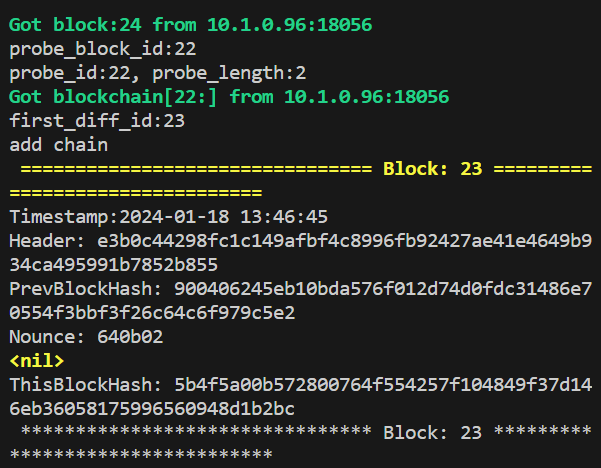
\includegraphics[width=0.9\textwidth]{./Exponential-search.png}
			\caption{figure for section 2}
		\end{figure}
		%\cite{}
		%%%%%%%%%%%%%%%%%%%%%%%%%%%%%%%%%%%%%%%%%%%%%%%%%%%%%%%%%%%%%
		% Begin edit from here
\end{spacing}
\end{document}
